\documentclass{article}
\usepackage{pgfplots}
\usepackage{pgfplotstable}
\pgfplotsset{compat=1.18}

\begin{document}

\begin{figure}[h]
\centering
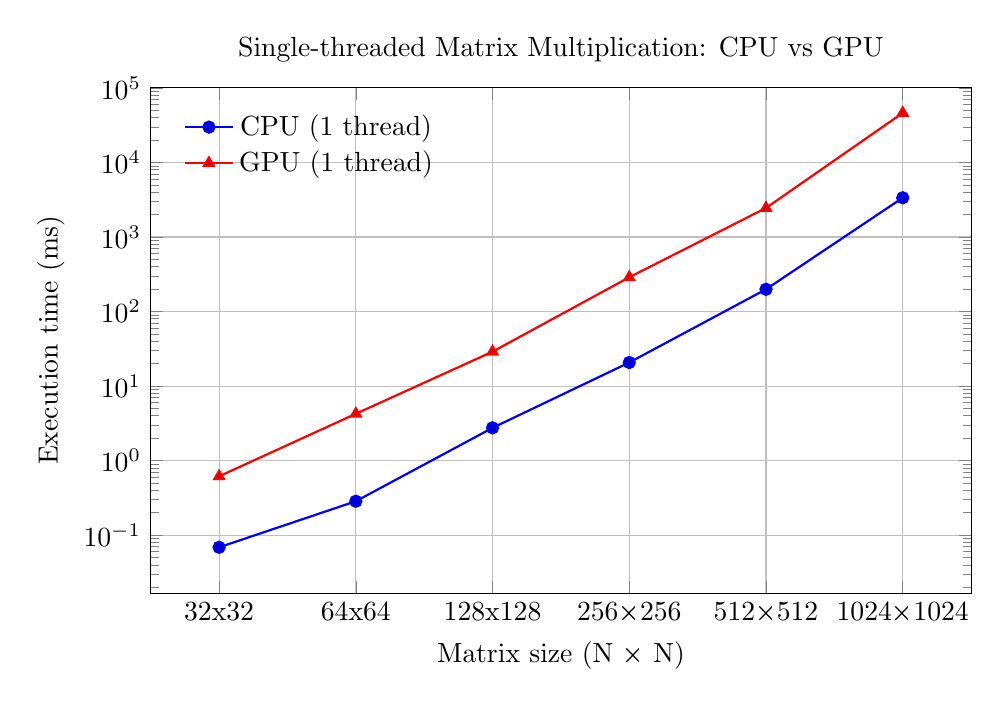
\begin{tikzpicture}
\begin{axis}[
    ymode=log,
    log basis y=10,
    width=12cm,
    height=8cm,
    xlabel={Matrix size (N × N)},
    ylabel={Execution time (ms)},
    title={Single-threaded Matrix Multiplication: CPU vs GPU},
    legend pos=north west,
    xtick=data,
    xticklabels={32x32, 64x64, 128x128, 256×256, 512×512, 1024×1024},
    ymin=0,
    ymax=100000,
    grid=major,
    legend style={draw=none, fill=none}
]

\addplot+[mark=*, thick, blue] coordinates {
    (1, 0.068705)
    (2, 0.285104)
    (3, 2.751817)
    (4, 20.706290)
    (5, 198.716200)
	(6, 3356.762000)
};
\addlegendentry{CPU (1 thread)}

\addplot+[mark=triangle*, thick, red] coordinates {
    (1, 0.615584)
    (2, 4.249685)
    (3, 28.923530)
    (4, 287.943700)
    (5, 2446.466000)
    (6, 46097.410000)
};
\addlegendentry{GPU (1 thread)}

\end{axis}
\end{tikzpicture}
\caption{Execution time of single-threaded CPU vs GPU matrix multiplication (log scale Y-axis)}
\end{figure}

\begin{tabular}{|r|r|r|r|r|}
\hline
\textbf{Matrix Size (n $\times$ n)} & \textbf{CPU Time (ms)} & \textbf{GPU Time (ms)} & \textbf{Speedup (GPU/CPU)} \\
\hline
32 $\times$ 32     & 0.068705   & 0.615584    & 11.970438 \\
64 $\times$ 64     & 0.285104   & 4.249685    & 15.554119 \\
128 $\times$ 128   & 2.751817   & 28.923530   & 11.419879 \\
256 $\times$ 256   & 20.706290  & 287.933700  & 13.906730 \\
512 $\times$ 512   & 198.716200 & 2446.466000 & 12.323010 \\
1024 $\times$ 1024 & 3356.762000 & 46097.410000 & 13.745850 \\
\hline
\end{tabular}

\end{document}

